\begin{center}
	\textbf{{\Huge ĐỀ 001}}
\end{center}
\subsubsection*{Phần I. Thí sinh trả lời từ câu 1 đến câu 12, mỗi câu hỏi chọn một phương án.}
\setcounter{bt}{0}\setlist[enumerate,1]{label=\quad\bfseries\Alph*.}
\begin{baitap}
	Cho hàm số có đồ thị như hình vẽ bên. Khẳng định nào sau đây là \textbf{đúng}?
	
	\begin{minipage}{0.6\textwidth}
		\begin{enumerate}[\quad \bf A.]
			\item Hàm số nghịch biến trên khoảng $(-\infty; 1)$.
			\item Hàm số nghịch biến trên khoảng $(-\infty; 0)$.
			\item Hàm số nghịch biến trên khoảng $\left(\frac{7}{3}; +\infty\right)$.
			\item Hàm số đồng biến trên khoảng $(-\infty; 1)$.
		\end{enumerate}
	\end{minipage}
	%	\vspace{2cm}
	\begin{minipage}{0.4\textwidth}
		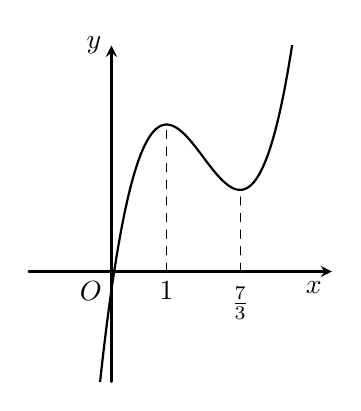
\begin{tikzpicture}[line cap=round, line join=round, >=stealth, scale=.7]
			% Define window bounds
			\def\xmin{-1.5} \def\xmax{4.0}
			\def\ymin{-2} \def\ymax{4.1}
			
			% Define exact fractions for critical points
			\pgfmathsetmacro{\xA}{1}
			\pgfmathsetmacro{\xB}{7/3}
			
			% Scope to clip the cubic function graph
			\begin{scope}
				\clip (\xmin,\ymin) rectangle (\xmax,\ymax);
				
				% Graph of f(x) = (x-1)^2 * (x - 3) + 3 = x^3 - 5x^2 + 7x - 2 + 2 = x^3 - 4.333x^2 + ...
				% Fits the shape: local max at x = 1, local min at x = 7/3
				\draw[black, thick, smooth, samples=200, domain=\xmin:\xmax]
				plot(\x, {(\x)^3 - 5*(\x)^2 + (63/9)*(\x) - 1/3});
			\end{scope}
			
			% Dashed lines for critical points x = 1 and x = 7/3
			\draw[dashed, thin] (\xA,0) -- (\xA, {(\xA)^3 - 5*(\xA)^2 + (63/9)*(\xA) - 1/3});
			\draw[dashed, thin] (\xB,0) -- (\xB, {(\xB)^3 - 5*(\xB)^2 + (63/9)*(\xB) - 1/3});
			
			% Draw Axes
			\draw[->, thick] (\xmin,0) -- (\xmax,0) node[below left]{$x$};
			\draw[->, thick] (0,\ymin) -- (0,\ymax) node[left]{$y$};
			
			% Labels on Axes
			\node[below left] at (0,0) {$O$};
			\node[below] at (\xA,0) {$1$};
			\node[below=2pt] at (\xB,0) {$\frac{7}{3}$};
		\end{tikzpicture}
	\end{minipage}
	%	\begin{multicols}{2}
		
		%	\end{multicols}
\end{baitap}
\begin{baitap}
	Cho hàm số $y = \dfrac{8 - 5x}{-4x - 9}$. Khẳng định nào sau đây là \textbf{sai}?
	\begin{multicols}{2}
		\begin{enumerate}[\quad \bf A.]
		\item Hàm số đồng biến trên khoảng $\left(-\infty; -\frac{37}{4}\right)$.
		\item Hàm số đồng biến trên khoảng $\left(-\infty; -\frac{9}{4}\right)$.
		\item Hàm số đồng biến trên khoảng $\left(-\frac{9}{4}; +\infty\right)$.
		\item Hàm số nghịch biến trên khoảng $\left(-\infty; -\frac{37}{4}\right)$.
	\end{enumerate}
	\end{multicols}
\end{baitap}

\begin{baitap}
	Cho hàm số có bảng biến thiên như sau
	\begin{center}
		
\begin{tikzpicture}[scale=.8]
			\tkzTabInit[lgt=1.5, espcl=3]{$x$ / 1, $y'$ / 1, $y$ / 2.5}{$-\infty$, $-\frac{4}{3}$, $\frac{1}{2}$, $+\infty$}
			\tkzTabLine{, +, 0, -, 0, +, }
			\tkzTabVar{-/ $-\infty$, +/ $\frac{218}{27}$, -/ $\frac{-17}{4}$, +/ $+\infty$}
		\end{tikzpicture}
	\end{center}
	
	Khẳng định nào sau đây là \textbf{đúng}?
	\begin{multicols}{2}
		\begin{enumerate}[\quad \bf A.]
		\item Hàm số nghịch biến trên khoảng $\left(-\infty; -\frac{4}{3}\right)$.
		\item Hàm số đồng biến trên khoảng $\left(-\frac{4}{3}; \frac{1}{2}\right)$.
		\item Hàm số nghịch biến trên khoảng $\left(\frac{7}{2}; +\infty\right)$.
		\item Hàm số đồng biến trên khoảng $\left(-\infty; -\frac{7}{3}\right)$.
	\end{enumerate}
	\end{multicols}
\end{baitap}

\begin{baitap}
%	\textbf{Câu 2.} TẠ QUANG BƯỬ
	Cho hàm số $f(x)$ liên tục trên $ \mathbb{R} $ và có đạo hàm $f'(x)=(x-1)^2(2-x)$. Hàm số $f(x)$ đồng biến trên khoảng nào?
	\begin{multicols}{4}
		\begin{enumerate}[\quad \bf A.]
			\item $(-1;3)$.
			\item $(2;+\infty)$.
			\item $(-\infty;2)$.
			\item $(2;5)$.
		\end{enumerate}
	\end{multicols}
\end{baitap}
\begin{baitap}
	Tìm tất cả các giá trị thực của tham số $m$ để hàm số $y = -\frac{1}{3}x^3 - mx^2 + (2m - 3)x - m + 2$ nghịch biến trên $\mathbb{R}$.
	\begin{multicols}{4}
		\begin{enumerate}[\quad \bf A.]
			\item $m \le -3$, $m \ge 1$.
			\item $-3 < m < 1$.
			\item $-3 \le m \le 1$.
			\item $m \le 1$.
		\end{enumerate}
	\end{multicols}
\end{baitap}

\begin{baitap}
	Cho hàm số $y = -x^3 - mx^2 + (4m + 9)x + 5$, với $m$ là tham số thực. Có bao nhiêu giá trị nguyên của $m$ để hàm số nghịch biến trên $(-\infty; +\infty)$?
	\begin{multicols}{4}
		\begin{enumerate}[\quad \bf A.]
			\item $5$.
			\item $6$.
			\item $7$.
			\item $4$.
		\end{enumerate}
	\end{multicols}
\end{baitap}

\begin{baitap}
	Cho hàm số $y = 7x^3 + 9x^2 - 3x - 4$. Khẳng định nào sau đây là \textbf{sai}?
	\begin{multicols}{2}
		\begin{enumerate}[\quad \bf A.]
			\item Giá trị cực đại $y = 1$.
			\item Hàm số đạt cực tiểu tại $x = \frac{1}{7}$.
			\item Giá trị cực tiểu $y = \frac{1}{7}$.
			\item Hàm số đạt cực đại tại $x = -1$.
		\end{enumerate}
	\end{multicols}
\end{baitap}

\begin{baitap}
	Cho hàm số $y = f(x)$ xác định trên $\mathbb{R}$ và có bảng biến thiên như hình vẽ sau:
	\begin{center}	
		
\begin{tikzpicture}[scale=.7]
			% Variation table based on the provided image
			\tkzTabInit[lgt=1.2, espcl=3]
			{$x$ / 1, $y'$ / 1, $y$ / 2.5}
			{$-\infty$, $10$, $12$, $+\infty$}
			
			\tkzTabLine{, +, z, -, z, +, }
			
			\tkzTabVar{-/$-\infty$, +/$-3$, -/$3$, +/$-\infty$}
		\end{tikzpicture}
%		\begin{tabular}{|c|ccccccc|}
%			\hline
%			$x$ & $-\infty$ & & $10$ & & $12$ & & $+\infty$ \\
%			\hline
%			$y'$ & & $+$ & $0$ & $-$ & $0$ & $+$ & \\
%			\hline
%			& & & $-3$ & & & & $-\infty$ \\
%			$y$ & & $\nearrow$ & & $\searrow$ & & $\nearrow$ & \\
%			& $-\infty$ & & & & $3$ & & \\
%			\hline
%		\end{tabular}
	\end{center}
	
	Hàm số $y = f(x)$ đạt cực đại tại
	\begin{multicols}{4}
		\begin{enumerate}[\quad \bf A.]
			\item $x = 10$.
			\item $x = 8$.
			\item $x = 12$.
			\item $x = 17$.
		\end{enumerate}
	\end{multicols}
\end{baitap}

%\begin{baitap}
%	\textbf{Câu 8.} Cho hàm số có đồ thị như hình bên. Khẳng định nào \textbf{sai}?
%	\begin{enumerate}[A.]
%		\item Hàm số có một cực tiểu tại $x = \dfrac{3}{4}$ và đạt cực đại tại $x = 0$.
%		\item Giá trị cực đại $y = -1$ và giá trị cực tiểu $y = -\dfrac{113}{32}$.
%		\item Hàm số có một cực tiểu tại $x = -\dfrac{3}{4}$.
%		\item Hàm số có một cực đại tại $x = -\dfrac{3}{4}$.
%	\end{enumerate}
%\end{baitap}

\begin{baitap} %Đề 001_de-khao-sat-chat-luong-toan-12-nam-2026-2027-truong-ta-quang-buu-ha-noi
	Cho hàm số $y=f(x)$ xác định trên tập $\mathbb{R}$ và có đồ thị như hình bên. Mệnh đề nào dưới đây đúng?
	\begin{minipage}{0.65\textwidth}
		\begin{enumerate}[\quad \bf A.]
			\item Hàm số đạt cực đại tại $x=0$ và đạt cực tiểu tại $x=2$.
			\item Hàm số có giá trị lớn nhất bằng $2$ và giá trị nhỏ nhất bằng $-2$.
			\item Hàm số có giá trị cực tiểu bằng $2$.
			\item Hàm số có ba điểm cực trị.
		\end{enumerate}
	\end{minipage}
	\begin{minipage}{0.35\textwidth}
		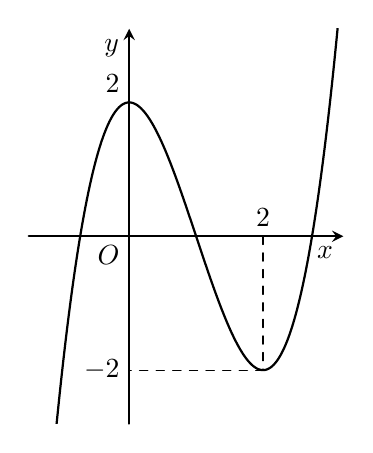
\begin{tikzpicture}[line cap=round, line join=round, >=stealth, scale=0.85]
			% Define plotting domain and bounding box
			\def\xmin{-1.5} \def\xmax{3.2}
			\def\ymin{-2.8} \def\ymax{3.1}
			
			% Function definition: cubic f(x) = x^3 - 3x^2 + 2
			% Local max at (0, 2), Local min at (2, -2)
			
			% Scope to clip the cubic curve safely within bounds
			\begin{scope}
				\clip (\xmin,\ymin) rectangle (\xmax,\ymax);
				
				% Graph of f(x) = x^3 - 3x^2 + 2
				\draw[black, thick, smooth, samples=200, domain=\xmin:\xmax]
				plot(\x, {(\x)^3 - 3*(\x)^2 + 2});
			\end{scope}
			
			% Dashed lines connecting critical point (2, -2) to axes
			\draw[dashed, thin] (2,0) -- (2,-2) -- (0,-2);
			
			% Draw Coordinate Axes (drawn on top of the curve)
			\draw[->, thick] (\xmin,0) -- (\xmax,0) node[below left]{$x$};
			\draw[->, thick] (0,\ymin) -- (0,\ymax) node[below left]{$y$};
			
			% Key Labels & Values
			\node[below left] at (0,0) {$O$};
			\node[above left] at (0,2) {$2$};
			\node[left] at (0,-2) {$-2$};
			\node[above] at (2,0) {$2$};
		\end{tikzpicture}
	\end{minipage}
\end{baitap}
\begin{baitap}
%	\textbf{Câu 10.} 
	Tìm tất cả các giá trị thực của $m$ để hàm số $y=x^3-3x^2+(m+1)x+2$ có hai điểm cực trị.
	\begin{multicols}{4}
		\begin{enumerate}[\quad \bf A.]
			\item $m < 2$.
			\item $m \le 2$.
			\item $m > 2$.
			\item $m < -4$.
		\end{enumerate}
	\end{multicols}
\end{baitap}

\begin{baitap}
%	\textbf{Câu 11.} 
	Cho hàm số $y=x^3-2mx^2+\left(-\frac{4}{3}m^2-40m-144\right)x-5$ ($m$ là tham số thực). Tìm tất cả các giá trị của $m$ để hàm số có cực trị?
	\begin{multicols}{2}
		\begin{enumerate}[\quad \bf A.]
			\item $-11 < m < -6$.
			\item $m < -9$ hoặc $m > -4$.
			\item $-14 < m < -6$.
			\item $m < -9$ hoặc $m > -6$.
		\end{enumerate}
	\end{multicols}
\end{baitap}
\begin{baitap}
	%	\textbf{Câu 9.} 
	Cho hàm số $y=8x^3-6mx^2+9mx+6m$ ($m$ là tham số thực). Giá trị của $m$ để hàm số đạt cực tiểu tại $x=-6$ thuộc khoảng nào sau đây?
	\begin{multicols}{4}
		\begin{enumerate}[\quad \bf A.]
			\item $\left(-\infty; -\frac{35}{3}\right)$.
			\item $\left(-\infty; -\frac{47}{3}\right)$.
			\item $\left(-\frac{23}{3}; +\infty\right)$.
			\item $\varnothing$.
		\end{enumerate}
	\end{multicols}
\end{baitap}
%\begin{baitap}
%	\textbf{Câu 12.} Cho hàm số $y=(m+1)x^4-mx^2+3$. Tìm tất cả các giá trị thực của tham số $m$ để hàm số có ba điểm cực trị.
%	\begin{multicols}{2}
%		\begin{enumerate}[\quad \bf A.]
%			\item $m \in (-\infty; -1) \cup [0; +\infty)$.
%			\item $m \in (-1; 0)$.
%			\item $m \in (-\infty; -1] \cup [0; +\infty)$.
%			\item $m \in (-\infty; -1) \cup (0; +\infty)$.
%		\end{enumerate}
%	\end{multicols}
%\end{baitap}


\subsubsection*{Phần II. Thí sinh trả lời từ câu 1 đến câu 4, trong ý a), b), c), d) ở mỗi câu câu, thí sinh chọn ĐÚNG hoặc SAI.}
\setcounter{bt}{0}\setlist[enumerate,1]{label=\quad\bfseries\alph*)}
\begin{baitap} %Câu 1 BGD Lần 1 2026
	Cho hàm số $f(x)=\dfrac{1}{3}x^3-5x^2+9x+8$
	\begin{enumerate}[\quad \bf a)]
		\item Hàm số đã cho có đạo hàm là $f'(x)=x^2-10x+9$.
		\item Phương trình $f'(x)=0$ có tập nghiệm là $S=\{1;9\}$.
		\item Hàm số đã cho nghịch biến trên khoảng $(1;9)$.
		\item Giá trị cực tiểu của hàm số đã cho bằng $\frac{37}{3}$.
	\end{enumerate}
\end{baitap}
\begin{baitap}
%	\textbf{Câu 1.} 
	Cho hàm số $f(x)=2x-4+\dfrac{2}{x+1}$.
	\begin{enumerate}[\quad \bf a)]
		\item Hàm số có đạo hàm $f'(x)=\dfrac{2(x^2+2x)}{(x+1)^2}$.
		\item Giá trị nhỏ nhất của hàm số trên khoảng $(-1;+\infty)$ bằng $-2$.
		\item Điểm cực đại của đồ thị hàm số có tọa độ $(0;-2)$.
		\item Hàm số $y=f(x)$ có tập xác định là $D=\mathbb{R} \setminus \{-1\}$.
	\end{enumerate}
\end{baitap}
\begin{baitap}
	Cho hàm số $f(x)=x^3-3x^2-1$.
	\begin{enumerate}[\quad \bf a)]
		\item Hàm số đã cho nghịch biến trên $\mathbb{R}$.
		\item Hàm số đã cho đồng biến trên $(3;+\infty)$.
		\item Hàm số đã cho nghịch biến trên $(1;2)$.
		\item Hàm số $g(x)=f(x)+2$ đồng biến trên $(-\infty;0)$.
	\end{enumerate}
\end{baitap}


\begin{baitap}
%	\textbf{Câu 2.} 
	Cho hàm số $y=f(x)$ có đồ thị như hình vẽ bên.
	
	\begin{minipage}{0.6\textwidth}
		\begin{enumerate}[\quad \bf a)]
		\item Hàm số đã cho nghịch biến trên khoảng $(-2,0)$.
		\item Hàm số đã cho đồng biến trên khoảng $(-3;1)$.
		\item Hàm số đã cho đồng biến trên khoảng $(2;+\infty)$.
		\item Hàm số $f=|f(x)|$ nghịch biến trên khoảng $(-2,0)$.
	\end{enumerate}
\end{minipage}
	\begin{minipage}{0.4\textwidth}
	% Cubic function y = x^3 + 3*x^2 - 1 with local max at (-2,3) and local min at (0,-1)
	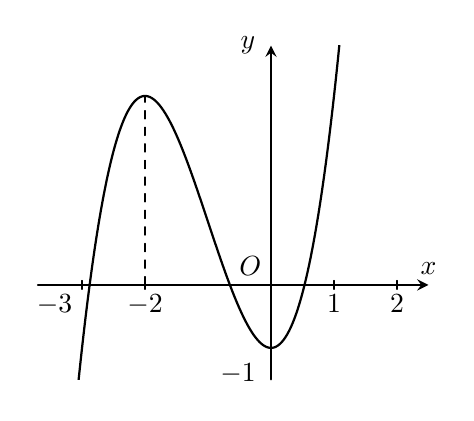
\begin{tikzpicture}[line cap=round, line join=round, >=stealth, scale=.8]
		% Bounding box definition
		\def\xmin{-3.7} \def\xmax{2.5}
		\def\ymin{-1.5} \def\ymax{3.8}
		
		% Scope to clip the curve within window bounds
		\begin{scope}
			\clip (\xmin,\ymin) rectangle (\xmax,\ymax);
			
			% Graph of cubic polynomial f(x) = x^3 + 3*x^2 - 1
			\draw[black, thick, smooth, samples=200, domain=\xmin:\xmax]
			plot(\x, {(\x)^3 + 3*(\x)^2 - 1});
		\end{scope}
		
		% Dashed line connecting local max (-2,3) to x-axis
		\draw[dashed, thin] (-2,0) -- (-2,3);
		
		% Draw Coordinate Axes (drawn on top of curve)
		\draw[->, thick] (\xmin,0) -- (\xmax,0) node[above]{$x$};
		\draw[->, thick] (0,\ymin) -- (0,\ymax) node[left=2pt]{$y$};
		
		% Origin label
		\node[above left] at (0,0) {$O$};
		
		% Tick marks and labels on X-axis
		\foreach \x in {-3,-2,1,2} {
			\draw (\x, 2pt) -- (\x, -2pt);
		}
		\node[below left] at (-3,0) {$-3$};
		\node[below] at (-2,0) {$-2$};
		\node[below] at (1,0) {$1$};
		\node[below] at (2,0) {$2$};
		
		% Y-axis value label (-1 at local minimum)
		\node[below left=2pt] at (0,-1) {$-1$};
	\end{tikzpicture}
	\end{minipage}
\end{baitap}



\subsubsection*{Phần III. Thí sinh trả lời từ câu 1 đến câu 6 (không làm tròn các phép tính trung gian trong các câu từ 1 đến câu 6).}
\setcounter{bt}{0}
\begin{baitap}
%	\textbf{Câu 1.} 
	Cho hàm số $y = 4x^3 + 8x^2 - 3x + 3$. Giá trị cực đại của hàm số bằng bao nhiêu?
\end{baitap}

\begin{baitap}
%	\textbf{Câu 2.} 
	Điểm cực tiểu của hàm số $y = x^3 - 5x^2 - 8x + 8$ bằng bao nhiêu?
\end{baitap}

\begin{baitap}
	Một chuyển động có vận tốc được xác định bởi phương trình $v(t) = -t^2 + 3t - 2$ với $t \ge 0$, trong đó $t$ tính bằng giây và $v$ tính bằng $\si{m/s}$. Kể từ giây thứ bao nhiêu trở đi thì vận tốc của vật giảm?
\end{baitap}

\begin{baitap}
	Cho hàm số $y = x^3 - 4x^2 + 5x + 2$. Hàm số có điểm cực đại và điểm cực tiểu lần lượt là $x_1, x_2$. Tính giá trị biểu thức $A = x_1 - 3x_2$.
\end{baitap}


\begin{baitap}
	Cho hàm số $y = -x^3 - mx^2 + (4m + 9)x + 3$ với $m$ là tham số. Có bao nhiêu giá trị nguyên của $m$ để hàm số nghịch biến trên $(-\infty; +\infty)$?
\end{baitap}

\begin{baitap}
	Đồ thị hàm số $y = x^3 - 3x^2 + 2ax + b$ có điểm cực tiểu $A(2; -2)$. Khi đó $a + b$ bằng bao nhiêu?
\end{baitap}

%\begin{baitap}
%	Có bao nhiêu giá trị nguyên của tham số $m$ để hàm số $y = x^3 - 3(m + 2)x^2 + 3(m^2 + 4m)x + 1$ nghịch biến trên khoảng $(0; 1)$?
%\end{baitap}
